% !TeX program = lualatex
% !BIB program = biber
% Lualatex is important to render Fira fonts; with pdflatex it's just the regular one
% ratio 16:9 -- https://tex.stackexchange.com/questions/14336/

% compile two versions, inspired by https://tex.stackexchange.com/a/1501
% use the script "compile-pdf.sh"
\newif\ifhandout
% if flags.tex does not exist, create an empty file to be able to compile in TeXstudio
\input{flags}

\ifhandout
	\documentclass[12pt,aspectratio=169,handout]{beamer}
\else
	\documentclass[12pt,aspectratio=169]{beamer}
\fi

% adjust for 16:9
% https://tex.stackexchange.com/questions/354022/modifying-the-margins-of-all-slides-in-beamer
\setbeamersize{text margin left=0.3cm,text margin right=1.0cm} 

%\usepackage{xcolor}

%%% better TOC
\usetheme[subsectionpage=progressbar]{metropolis}

% name in footer
\setbeamertemplate{frame numbering}{\insertframenumber ~ | Dr.\ Martin Tutek}

% blocks with background globally
\metroset{block=fill}

% adjust the background to be completely white
\setbeamercolor{background canvas}{bg=white}

% typeset mathematics on serif
\usefonttheme[onlymath]{serif}

% better bibliography using biber as backend
\usepackage[natbib=true,backend=biber,style=authoryear-icomp,maxbibnames=30,maxcitenames=2,uniquelist=false,giveninits=true,doi=false,url=false,dashed=false,isbn=false]{biblatex}
% shared bibliography
\addbibresource{../dl4nlp-bibliography.bib}
% disable "ibid" for repeated citations
\boolfalse{citetracker}

\definecolor{76abdf}{RGB}{118, 171, 223}

\setbeamercolor{frametitle}{bg=76abdf, fg=white}

\newcounter{saveenumi}
\newcommand{\seti}{\setcounter{saveenumi}{\value{enumi}}}
\newcommand{\conti}{\setcounter{enumi}{\value{saveenumi}}}

\resetcounteronoverlays{saveenumi}
% \usepackage{movie15}
\usepackage{animate}

\usepackage{xspace}
% Emojis
\usepackage{emoji}
% Figs
\usepackage{graphicx}
\graphicspath{ {./img/} }


% for derivatives, https://tex.stackexchange.com/a/412442
\usepackage{physics}

\usepackage{tikz}
\usetikzlibrary{matrix, positioning}
\usetikzlibrary{angles,quotes} % for angles
\usetikzlibrary{backgrounds} % background
\usetikzlibrary{decorations.pathreplacing} % curly braces
\usetikzlibrary{calligraphy}
\usetikzlibrary{calc} % for neural nets

% for plotting functions
\usepackage{pgfplots}
\usepgfplotslibrary{dateplot}

% sub-figures
\usepackage{caption}
\usepackage{subcaption}

% Checkmark, xmark
\usepackage{pifont}% http://ctan.org/pkg/pifont

% book tabs
\usepackage{booktabs}

% caption*
\usepackage{caption}


% show TOC at every section start
\AtBeginSection{
	\frame{
		\vspace{2em}
		\sectionpage
		\hspace*{2.2em}\begin{minipage}{10cm}
			\tableofcontents[currentsection]
		\end{minipage}
	}
}

% argmin, argmax
\usepackage{amssymb}% http://ctan.org/pkg/amssymb
\usepackage{amsmath}

\DeclareMathOperator*{\argmax}{arg\!\max}
\DeclareMathOperator*{\argmin}{arg\!\min}
% softmax
\DeclareMathOperator*{\softmax}{soft\!\max}
% RNN
\DeclareMathOperator*{\rnn}{RNN}
% RNN star
\DeclareMathOperator*{\rnnstar}{RNN^{*}}
% bi-RNN
\DeclareMathOperator*{\birnn}{biRNN}

% bold math
\usepackage{bm}

% for \mathclap
\usepackage{mathtools}

% algorithms
\usepackage[noend]{algpseudocode}


% for neurons and layers in tikz
\tikzset{
	neuron/.style={draw, rectangle, inner sep=2pt, minimum width=0.75cm, fill=blue!20},
	param/.style={draw, rectangle, inner sep=2pt, minimum width=0.75cm, fill=green!20},
	constant/.style={draw, rectangle, inner sep=2pt, minimum width=0.75cm, fill=black!15},
	state/.style={rectangle, inner sep=2pt, minimum width=0.75cm, fill=black!5},
}

% for strike-through text
\usepackage[normalem]{ulem}


\title{Deep Learning for Natural Language Processing}
\subtitle{Lecture 11 -- Text generation 4: Decoder-only Models and GPT}
\date{June 27, 2023}
\author{Dr.\ Martin Tutek}
\institute{Ubiquitous Knowledge Processing  \hfill 
\includegraphics[height=1.cm]{img/ukp_logo.png} \\
Department of Computer Science\\
Technical University of Darmstadt \hfill \href{https://www.informatik.tu-darmstadt.de/ukp/ukp_home/index.en.jsp}{\underline{UKP Web}}}
%\titlegraphic{\hfill }

\begin{document}

\maketitle

\begin{frame}{Recap}
	In the previous lecture we:
	\begin{itemize}
		\item Introduced the \textbf{BERT model}
		\item Introduced the two pretraining tasks for BERT: \textbf{MLM} and \textbf{NSP}
		\item Explained the connection between MLM and CBOW-style training
		\item Explained the purpose of NSP -- learning a \textbf{sentence embedding}
		\item Analyzed how to \textbf{apply BERT} to various \textbf{downstream tasks} such as classification and QA
		\item Gave an overview of various other pretraining tasks for LLMs
	\end{itemize}
\end{frame}

\begin{frame}{Motivation}
Recall: using the \textbf{same model} for \textbf{multiple tasks} without task-specific decoder heads
	\begin{figure}[h]
		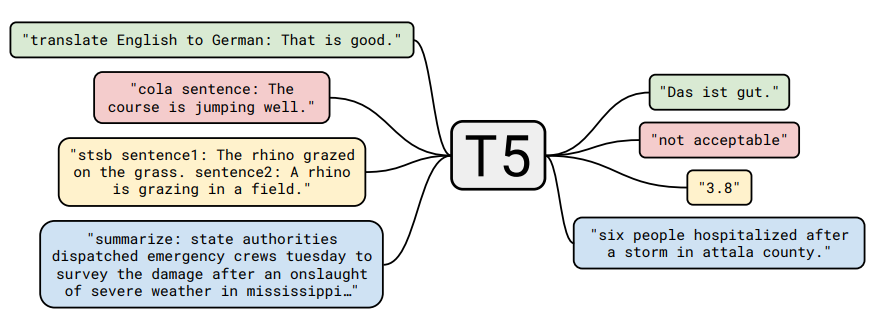
\includegraphics[height=4.5cm]{t5-objectives}
		\caption*{Image from \href{https://jmlr.org/papers/volume21/20-074/20-074.pdf}{\underline{T5 paper}}}
	\end{figure}
\end{frame}

\begin{frame}{Motivation}
	Recall: using the \textbf{same model} for \textbf{multiple tasks} without task-specific decoder heads
		\begin{figure}[h]
			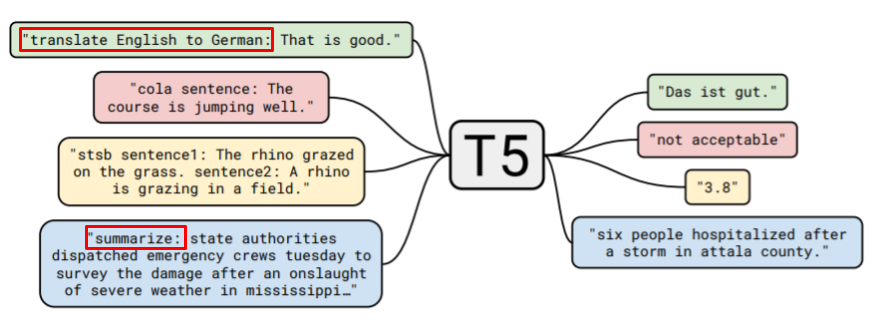
\includegraphics[height=4.5cm]{t5-anno-prompts}
			\caption*{Image from \href{https://jmlr.org/papers/volume21/20-074/20-074.pdf}{\underline{T5 paper}}}
		\end{figure}
	\end{frame}

\section{Types of Transformer Architectures}

\begin{frame}{Encoder-Decoder Transformer}

	\begin{figure}[h]
		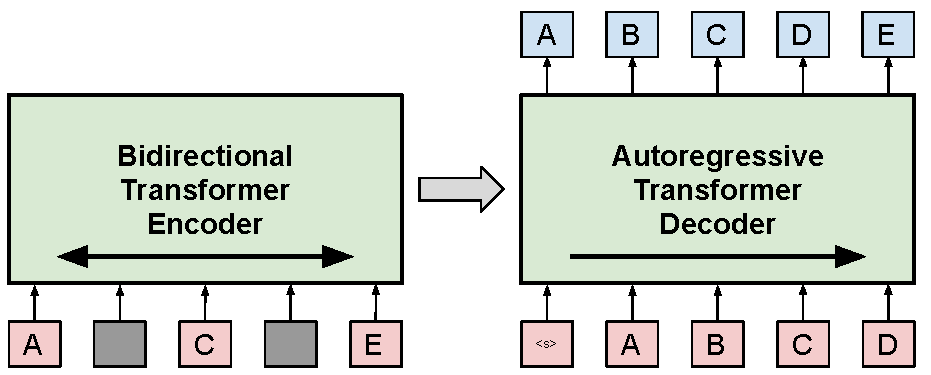
\includegraphics[height=4.5cm]{transformer_enc_dec.pdf}
	\end{figure}

\end{frame}


\begin{frame}{Bidirectional Encoder-only Transformer}
\begin{columns}[T] % align columns
	\begin{column}{.48\textwidth}
	\begin{figure}[h]
		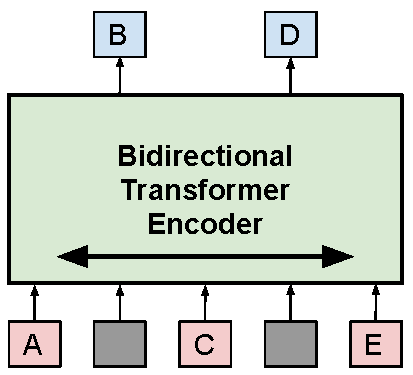
\includegraphics[height=4.5cm]{bidirectional_trf_encoder.pdf}
	\end{figure}
	\end{column}
	
	\begin{column}{.48\textwidth}
		\begin{itemize}
			\item Efficient encoding \emoji{check-mark}
			\item Versatile base for downstream tasks \emoji{check-mark}
			\pause
			\item Can't \textbf{really} generate text \emoji{cross-mark}
		\end{itemize}
	\end{column}

\end{columns}
\end{frame}


\begin{frame}{Autoregressive Decoder-only Transformer}
	\begin{columns}[T] % align columns
		\begin{column}{.48\textwidth}
	\begin{figure}[h]
		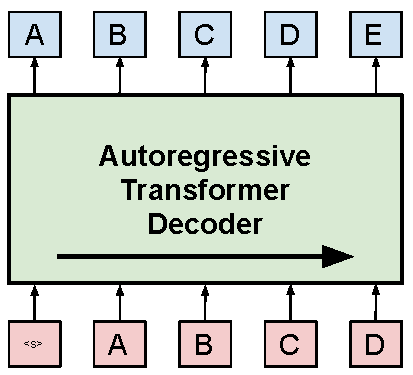
\includegraphics[height=4.5cm]{autoregressive_trf_decoder.pdf}
	\end{figure}
\end{column}
	
\begin{column}{.48\textwidth}
	An \textbf{autoregressive} (causal) language model uses \textbf{past} values of a time series to predict future values.
	\pause
	\begin{itemize}
		\item Didn't we decide not to use these because they were inefficient?
		\pause \begin{center} \textbf{(RNNs)} \end{center}
		\pause
		\item Yes, but... 
		\begin{enumerate}
			\item Hardware has improved
			\item Autoregressive models are \textit{really} good at generating text
		\end{enumerate}
	\end{itemize}
\end{column}
\end{columns}

\end{frame}

\begin{frame}{Differences between attention masks}
	\begin{figure}[h]
		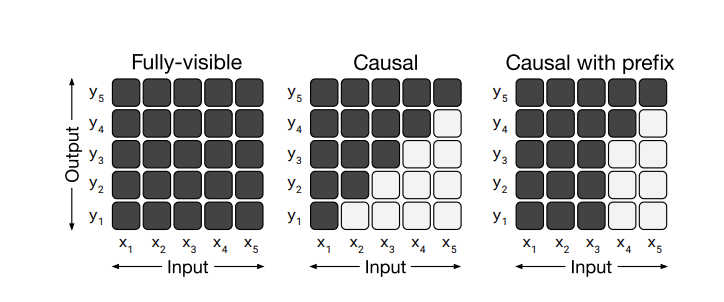
\includegraphics[height=4.5cm]{attention-types}
	\end{figure}
	Read: y axis $\to$ tokens attending, x axis $\to$ tokens attended to.
	
	Black cell $\to$ token visible, white cell $\to$ token \textbf{masked}
\end{frame}

\begin{frame}{Differences between attention masks}
	\begin{figure}[h]
		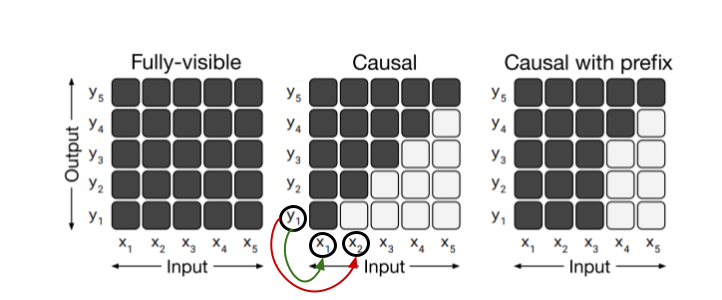
\includegraphics[height=4.5cm]{attention-masks-anno}
	\end{figure}
	Read: y axis $\to$ tokens attending, x axis $\to$ tokens attended to.
	
	Black cell $\to$ token visible, white cell $\to$ token \textbf{masked}
\end{frame}

\begin{frame}{Attention masks}

	Recall: the attention mechanism

	\noindent\begin{minipage}{0.4\textwidth}
		\begin{equation*}
			a = \sum_i^n \alpha_i v_i
		\end{equation*} 
	\end{minipage}%
	\begin{minipage}{0.2\textwidth}
	\end{minipage}
	\begin{minipage}{0.4\textwidth}
		\begin{equation*}
			\hat{\alpha}_i = \frac{q^T \cdot k_i}{\sqrt{d_{\text{model} } } }
		\end{equation*}
	\end{minipage}\vskip1em

	\pause
	How do we do \textbf{masking}?

	In the \textbf{causal} scenario (each token can only attend to \textbf{past} tokens);
	\pause
	
	For a $q = W_q(s_j)$ query computed based on the hidden state $s_j$ at position $j$
	\pause

	$$
		\alpha_i = 
		\begin{cases}
			\alpha_i,& \text{if } j\geq i\\
			0,              & \text{otherwise}
		\end{cases}
	$$
	\pause
	\textbf{NB: actually}, we set $\hat{\alpha}_i$ to $-\inf$ (before softmax) 

\end{frame}


\begin{frame}{Differences between attention masks}
	\begin{figure}[h]
		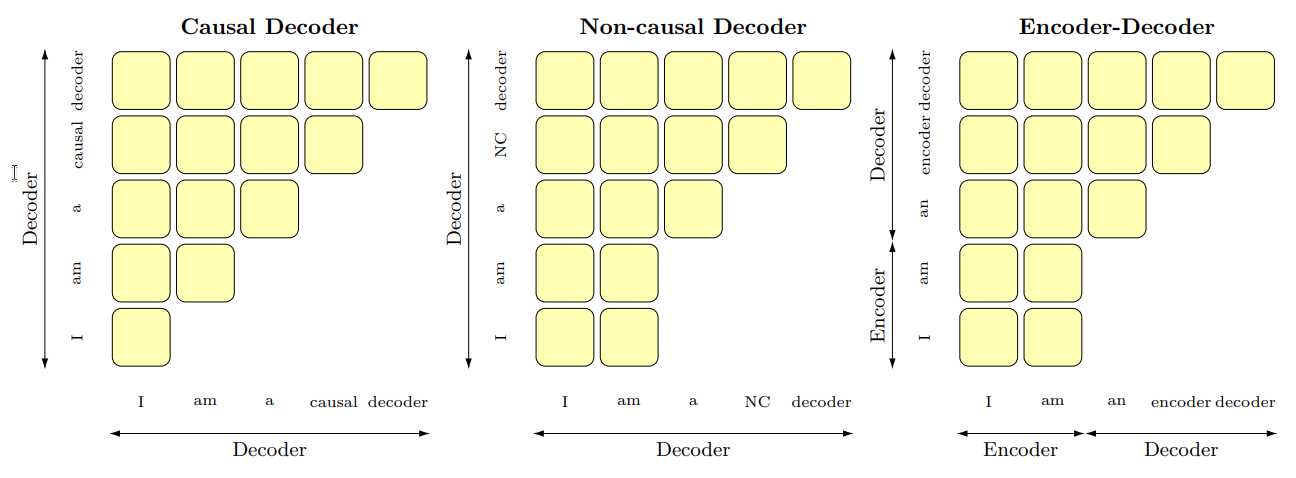
\includegraphics[height=5.5cm]{attention-patterns}
	\end{figure}
\end{frame}

\section{Autoregressive decoder-only Models}

\begin{frame}{Variants of language modeling}
	\begin{figure}[h]
		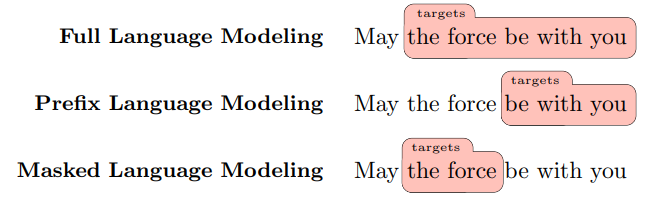
\includegraphics[height=3.5cm]{language-modeling-types}
	\end{figure}

	\begin{itemize}
		\item (Full) language modeling $\to$ given previous tokens, predict next token, for \textbf{every token} in sequence
		\pause
		\item Prefix language modeling $\to$ (1) feed a prefix (where mask \textbf{does not have to be causal}), (2) full LM starting after prefix
		\pause
		\item Masked language modeling $\to$ \textbf{reconstruct masked} tokens/spans
	\end{itemize}
	
\end{frame}

\begin{frame}{Autoregressive decoder-only models}
	\begin{figure}[h]
		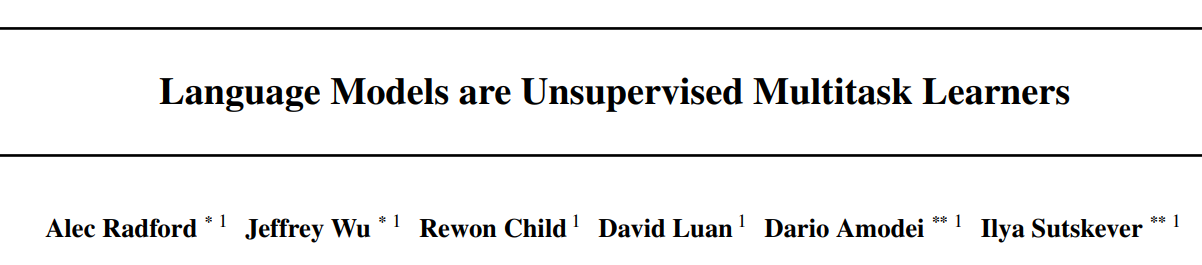
\includegraphics[height=3cm]{gpt2-paper}
	\end{figure}

	Introduction of \textbf{GPT-2}, an autoregressive Transformer decoder-only model trained on full language modeling.

	\pause

	\textbf{GPT-3} is \textit{"just"} a \textbf{larger} version of GPT-2 

\end{frame}

\begin{frame}{Autoregressive decoder-only models}
	\begin{figure}[h]
		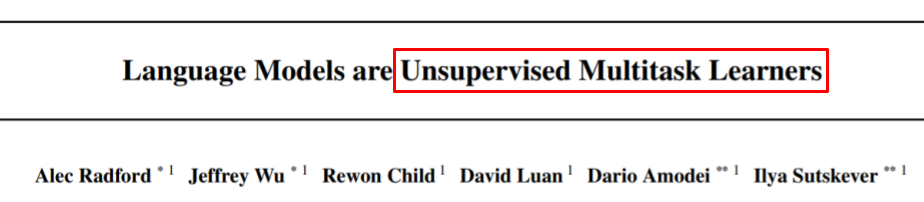
\includegraphics[height=3cm]{gpt2-title-anno}
	\end{figure}

	Introduction of \textbf{GPT-2}, an autoregressive Transformer decoder-only model trained on full language modeling.

	\hspace{1em} What does "unsupervised multitask learners" mean \emoji{thinking}?
\end{frame}

\subsection{Zero-shot, one-shot and few-shot learning}

\begin{frame}{Zero-shot, one-shot and few-shot learning}

\textbf{Recall:} T5 was able to perform \textbf{multiple tasks} at the same time

... but it was trained on them \& on keywords which indicate the task.
\vspace{1em}
\pause

For a model that has \textbf{not been trained on the downstream task}:
\begin{itemize}
	\item \textbf{Few-shot} learning: tune pretrained model on a \textbf{small number} of target task instances, \textbf{then perform task (!)}
	\pause
	\item \textbf{One-shot} learning: tune pretrained model on \textbf{one instance (!)} \textit{per class}, then perform task
	\pause
	\item \textbf{Zero-shot} learning: \textbf{don't tune pretrained model}\textbf{(!!!)}, then perform task 
\end{itemize}

\end{frame}

\begin{frame}{Zero-shot learning}
	Zero shot learning $\approx$ unsupervised learning
	\pause

	\vspace{1em}
	Why $\approx$?
	\pause

	\textbf{Assumption:} when trained on a \textbf{massive} corpus of text, the language model is likely to \textbf{see some tasks naturally} occur (e.g. question answering).

	\pause
	\begin{itemize}
		\item We want to \textbf{transform} our task into a \textbf{generative one} by providing a \textbf{prompt} to the model which will make the label of the input instance the \textbf{most likely generated sequence}.
	\end{itemize}
	
\end{frame}

\begin{frame}%{Zero-shot learning}
	\begin{columns}[T] % align columns
		\begin{column}{.48\textwidth}
	\begin{figure}[h]
		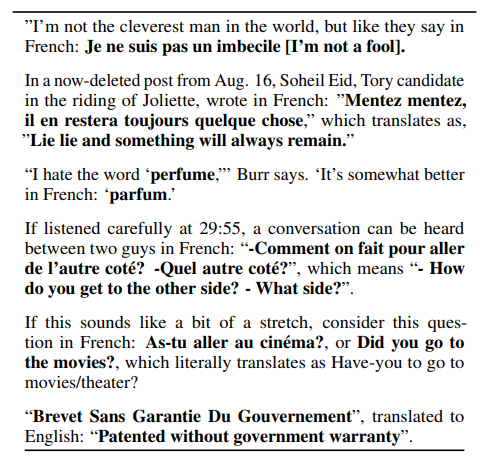
\includegraphics[height=7.3cm]{gpt2-demonstrations}
		\caption*{Image from \href{https://cdn.openai.com/better-language-models/language_models_are_unsupervised_multitask_learners.pdf}{\underline{GPT2 paper}}}
	\end{figure}
\end{column}
	
\begin{column}{.48\textwidth}
	\vspace{1.5em}
	The internet \textbf{does} contain samples of various NLP tasks
	\pause
	\begin{itemize}
		\item ... and a large language model (LLM) \textbf{can} remember them;
		\pause
		\item ... and when \textbf{prompted} to perform a task, without seeing the prompt before, \textbf{recall it};
		\pause
		\item ... and \textbf{perform them accurately}.
	\end{itemize}
\end{column}
\end{columns}
	
\end{frame}

\begin{frame}{GPT-2: Zero-shot question answering}
	\begin{figure}[h]
		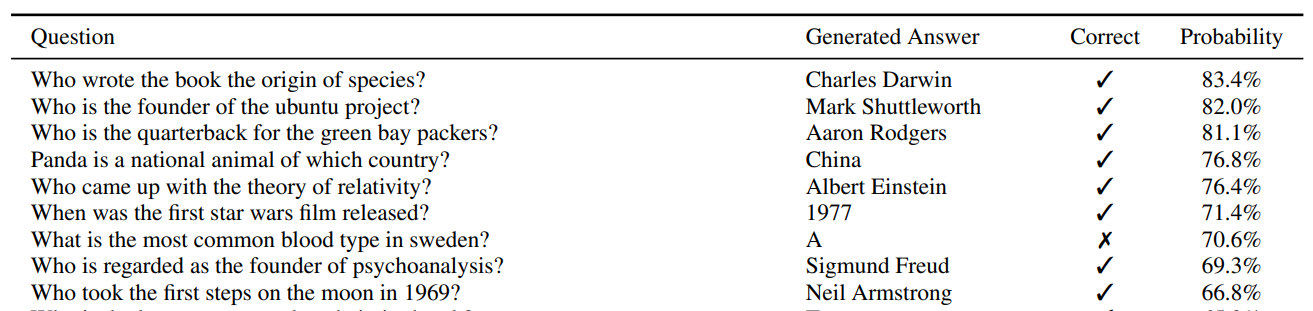
\includegraphics[height=3.5cm]{gpt2-zeroshot-qa}
		\caption*{Image from \href{https://cdn.openai.com/better-language-models/language_models_are_unsupervised_multitask_learners.pdf}{\underline{GPT2 paper}}}
	\end{figure}
\end{frame}


\begin{frame}{GPT-2: Prompted one-shot question answering}
	\begin{figure}[h]
		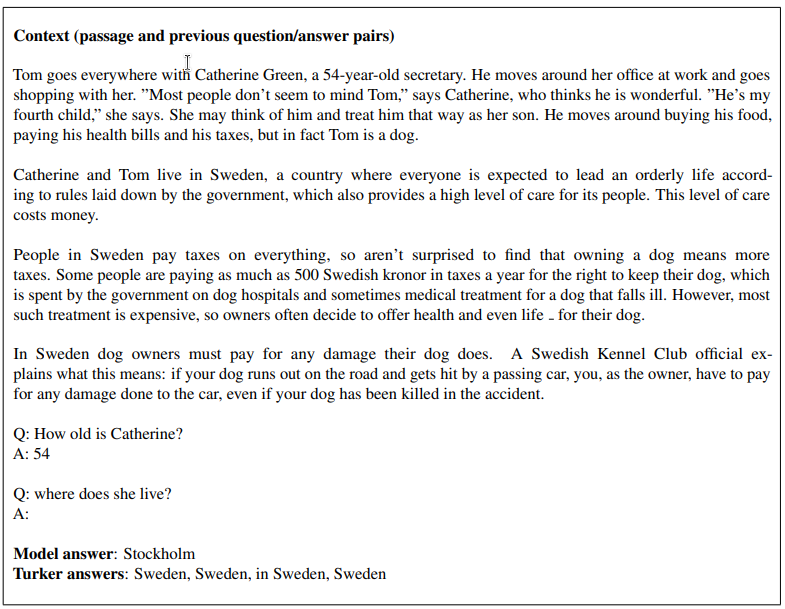
\includegraphics[height=6.5cm]{gpt2-prompting-qa}
		\caption*{Image from \href{https://cdn.openai.com/better-language-models/language_models_are_unsupervised_multitask_learners.pdf}{\underline{GPT2 paper}}}
	\end{figure}
\end{frame}

\begin{frame}
	\begin{figure}[h]
		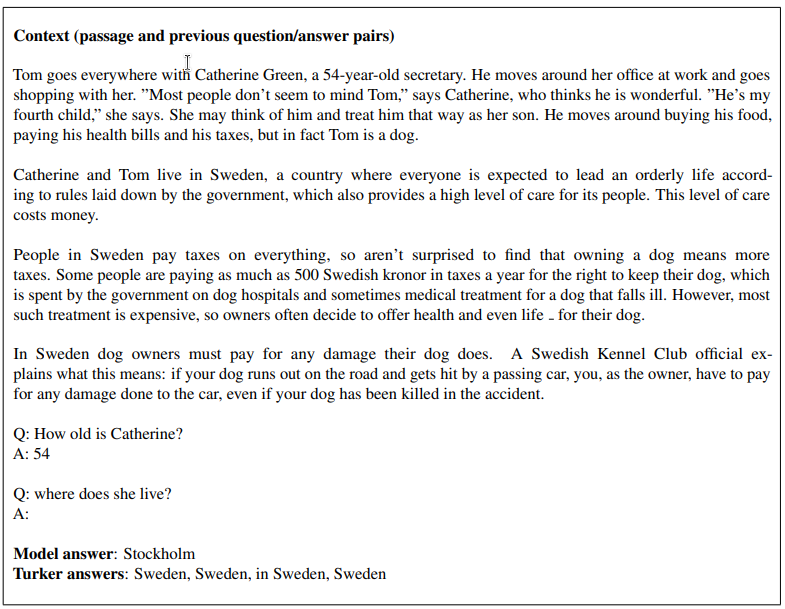
\includegraphics[height=8.5cm]{gpt2-prompting-qa}
		% \caption*{Image from \href{https://cdn.openai.com/better-language-models/language_models_are_unsupervised_multitask_learners.pdf}{\underline{GPT2 paper}}}
	\end{figure}
\end{frame}

\begin{frame}
	\begin{figure}[h]
		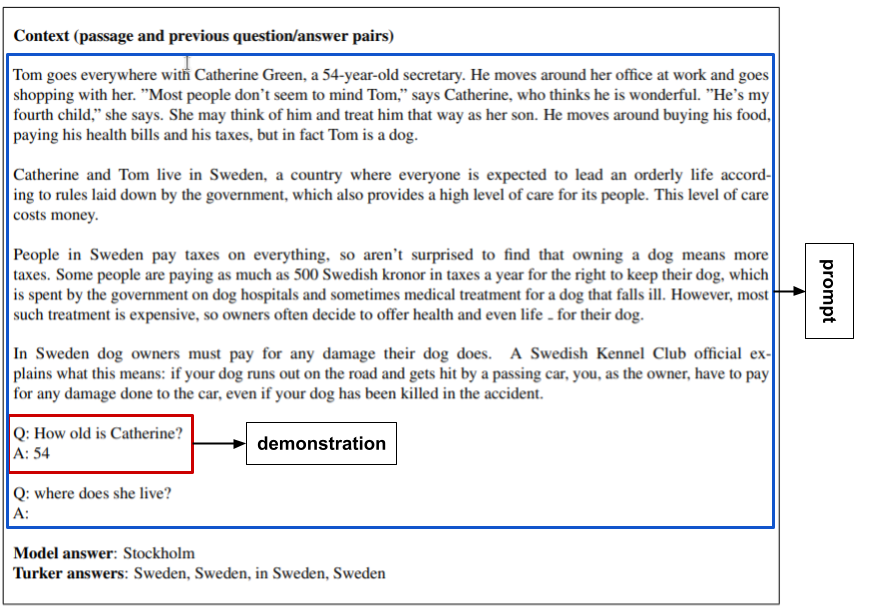
\includegraphics[height=8.5cm]{gpt2-prompt-anno}
		% \caption*{Image from \href{https://cdn.openai.com/better-language-models/language_models_are_unsupervised_multitask_learners.pdf}{\underline{GPT2 paper}}}
	\end{figure}
\end{frame}

\subsection{Prompting}

\begin{frame}{Prompting}
	\textbf{A prompt} is a piece of text inserted in the input examples, so that the original task \textbf{can be formulated as} a (masked) \textbf{language modeling} problem.

	\pause

	\begin{figure}[h]
		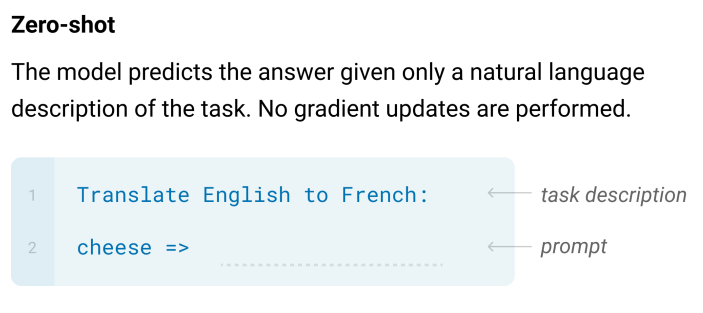
\includegraphics[height=5cm]{zero-shot-translation-gpt3}
		\caption*{Image from \href{https://arxiv.org/pdf/2005.14165.pdf}{\underline{GPT3 paper}}}
	\end{figure}
	
\end{frame}


\begin{frame}{Prompting}
	\textbf{A prompt} is a piece of text inserted in the input examples, so that the original task \textbf{can be formulated as} a (masked) \textbf{language modeling} problem.

	\begin{figure}[h]
		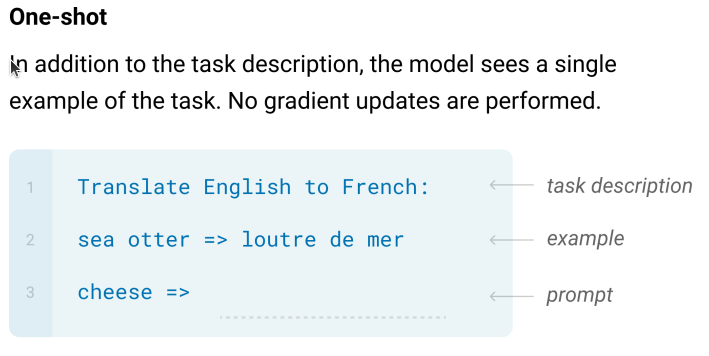
\includegraphics[height=5cm]{one-shot-translation-gpt3}
		\caption*{Image from \href{https://arxiv.org/pdf/2005.14165.pdf}{\underline{GPT3 paper}}}
	\end{figure}
	
\end{frame}


\begin{frame}{Prompting}
	\textbf{A prompt} is a piece of text inserted in the input examples, so that the original task \textbf{can be formulated as} a (masked) \textbf{language modeling} problem.

	\begin{figure}[h]
		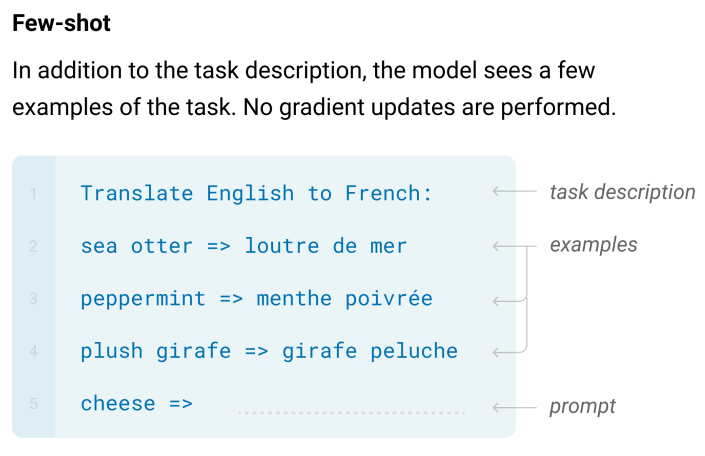
\includegraphics[height=5cm]{few-shot-translation-gpt3}
		\caption*{Image from \href{https://arxiv.org/pdf/2005.14165.pdf}{\underline{GPT3 paper}}}
	\end{figure}
	
\end{frame}

\begin{frame}{Prompting works well}
	\begin{figure}[h]
		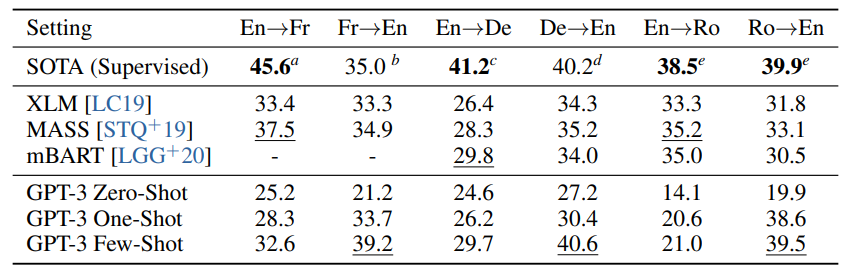
\includegraphics[height=4.5cm]{gpt3-translation-results}
		\caption*{Image from \href{https://arxiv.org/pdf/2005.14165.pdf}{\underline{GPT3 paper}}}
	\end{figure}
	GPT3 \textbf{without fine-tuning} performs better than \textbf{unsupervised} alternatives, and sometimes even \textbf{better} than supervised state-of-the-art!
\end{frame}

\begin{frame}{In-context learning}
	\textbf{In-context learning} is the paradigm in which a LLM learns to solve a new task at inference time \textbf{without any change to its weights}, based only on examples in the \textbf{prompt}.
	\pause

	\hspace{1em}$\approx$ umbrella term for zero-, one- and few-shot learning with task descriptions also contained in prompt.
	\vspace{1em}

	\pause
	\textit{"During \textbf{unsupervised pre-training}, a language model develops a broad set of skills and pattern recognition abilities. It then uses these abilities at inference time to rapidly adapt to or recognize the desired task. We use the term “in-context learning” to describe the inner loop of this process, which occurs \textbf{within the forward-pass} upon each sequence."} -- from GPT3 paper

\end{frame}

\begin{frame}%{In-context learning}
	\begin{figure}[h]
		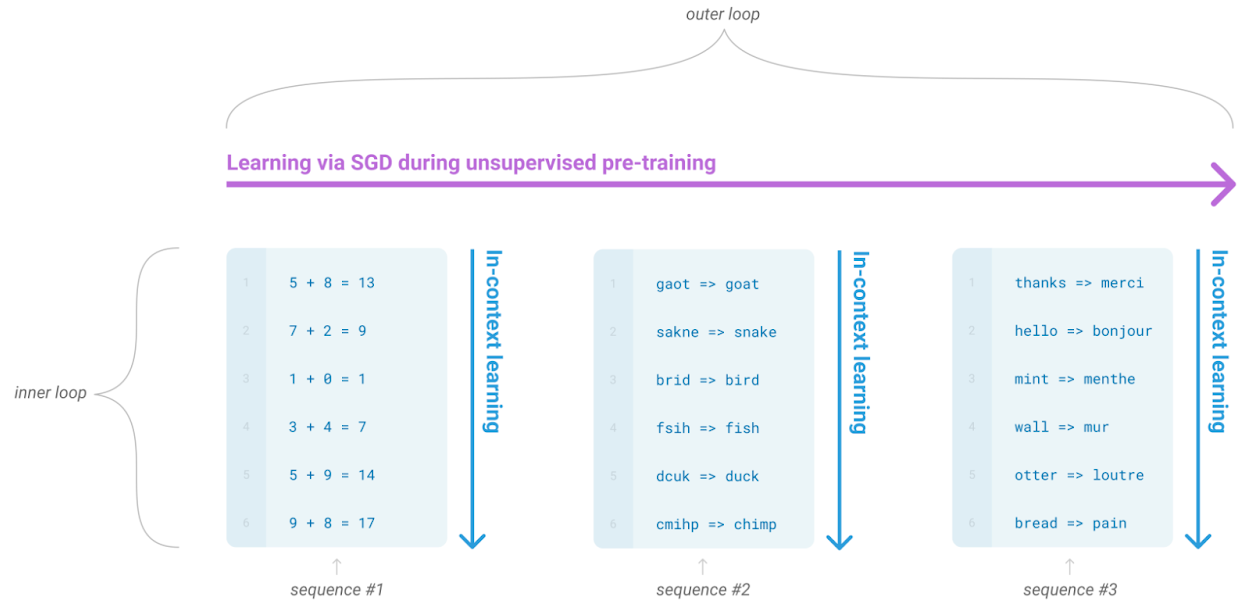
\includegraphics[height=7.5cm]{in-context-learning}
	\end{figure}

\end{frame}

\section{Prompt-tuning MLMs}

\begin{frame}{Prompt-tuning MLMs}
	Can we only use prompting with autoregressive models?
	\pause
	\vspace{1em}
	\begin{itemize}
		\item No -- we can also use it with bidirectional decoder-only models!
		\begin{itemize}
		\pause
		\item  ... but it is \textbf{more difficult} because they have not been trained to generate texts
		\pause
		\item ... because the downstream task is \textbf{less natural} (further from the pretraining task) to the model
		\end{itemize}

	\end{itemize}
	\pause
	How to overcome this gap between the \textbf{pretraining task} and the \textbf{prompting-transformed downstream task}?

\end{frame}

\begin{frame}{Prompt-tuning MLMs}
	So far, we have \textbf{fine-tuned} masked language models
	\pause
	\begin{figure}[h]
		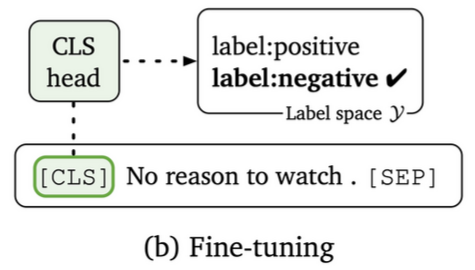
\includegraphics[height=4cm]{fine-tuning-mlms}
		\caption*{Figure from \href{https://thegradient.pub/prompting/}{\underline{The Gradient}}}
	\end{figure}
	\pause
	Can we frame our downstream task \textbf{as MLM}?

\end{frame}

\begin{frame}{Prompt-tuning MLMs}
	\begin{figure}[h]
		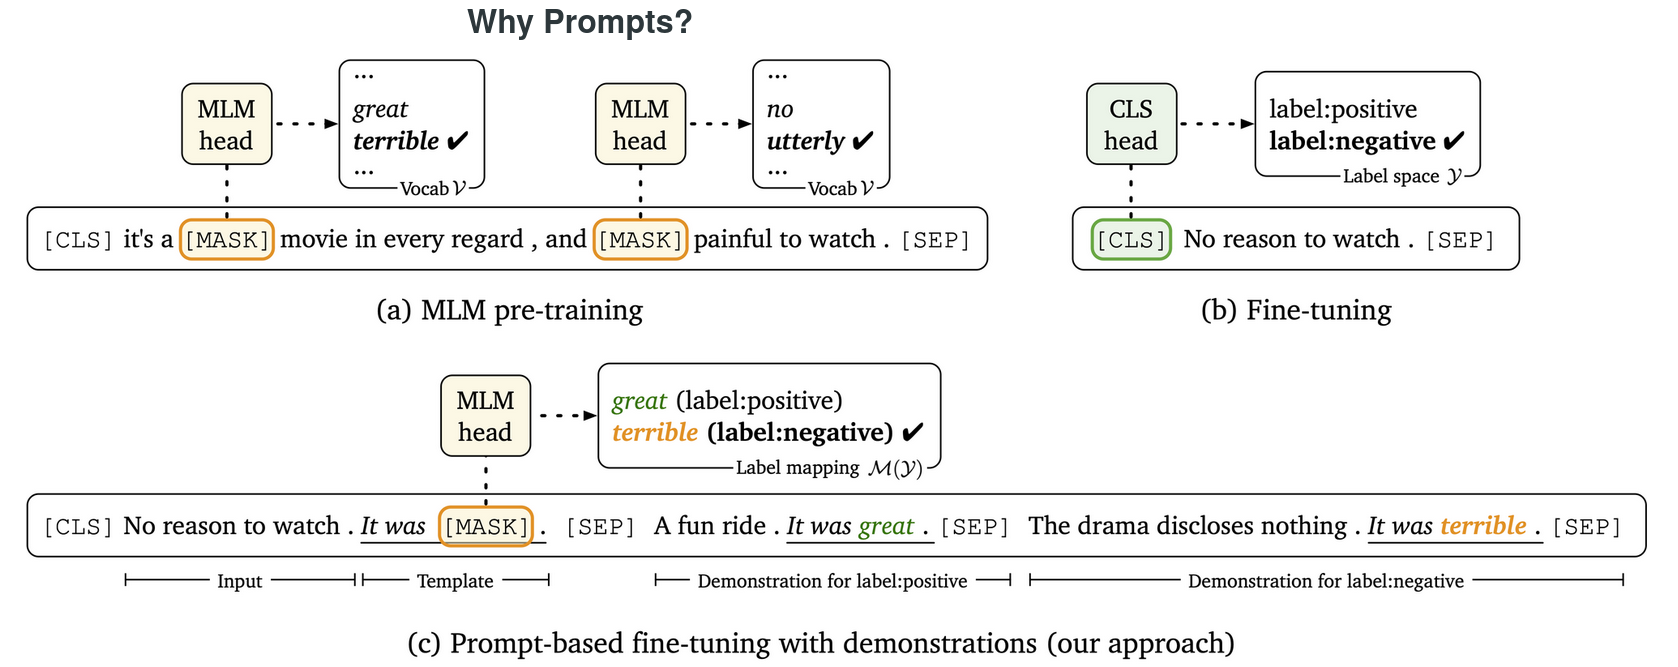
\includegraphics[height=6cm]{prompting_mlms}
	\end{figure}
\end{frame}


\begin{frame}{Prompt-tuning MLMs}
	We transform the target task (e.g. sentiment analysis) to \textbf{masked language modeling}.
	\begin{enumerate}
		\item Choose the prompt and word/token used for each label 
		\pause
		\begin{itemize}
			\item Choice of label token \textbf{important}
			\item Template design also \textbf{important}
		\end{itemize}
		\pause
		\item Demonstrate task through a few samples
		\pause
		\begin{itemize}
			\item Usually through \textbf{fine-tuning}
		\end{itemize}
		\pause
		\item \textbf{No new parameters needed} to perform task!
	\end{enumerate}
\end{frame}


\begin{frame}{Discrete and continuous prompts}
	So far, we have shown \textbf{discrete prompts}: actual text that we prepend/append to existing data which triggers the LLM to perform our task.
	\pause
	\vspace{1em}
	
	Can we learn \textbf{continuous prompts}? 
	\pause
	(dense vectors which we prepend, e.g. as a token)
	\pause
	\begin{figure}[h]
		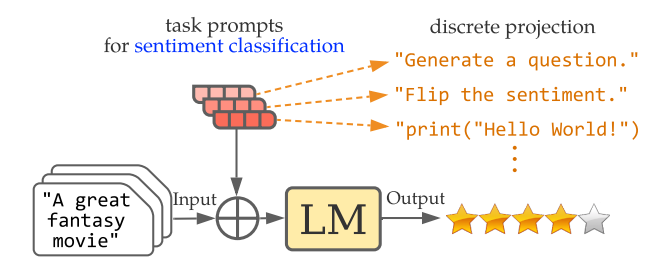
\includegraphics[height=3.5cm]{continuous-prompts}
		\caption*{Figure from \href{https://aclanthology.org/2022.naacl-main.266.pdf}{\underline{Prompt Waywardness}}}
	\end{figure}
\end{frame}


\section{A step back}

\begin{frame}{Incredible Performance of Large Language Models}
	So... what caused LLMs to be \textbf{so good} all of a sudden?
	\pause
	\begin{itemize}
		\item More available data (more data $\to$ better models)
		\pause
		\item Training tricks (from experience)
		\pause
		\item Hardware advancements (faster training of larger models)
	\end{itemize}
	\begin{figure}[h]
		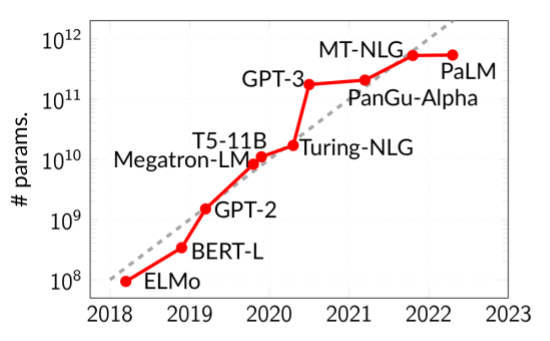
\includegraphics[height=4cm]{lm-scaling}
	\end{figure}
\end{frame}

\begin{frame}{Takeaways}
	
\begin{itemize}
	\item Three types of Transformer-based architectures for LLM pretraining:
	\begin{itemize}
		\item \textbf{Encoder-decoder} (T5)
		\item \textbf{Bidirectional encoder-only} (BERT)
		\item \textbf{Autoregressive decoder-only} (GPT-2)
	\end{itemize}
	\item The \textbf{attention masks} of these models differ
	\item There are three variants of language modeling for pretraining LLMs
	\item GPT-2 (and 3) are autoregressive decoder-only transformers
	\item We introduced zero-, one- and few-shot learning
	\item We introduced prompting and its variants
	\begin{itemize}
		\item Autoregressive vs MLM prompting
		\item Continuous vs discrete prompts
		\item In-context learning
	\end{itemize}
\end{itemize}
	
\end{frame}

\begin{frame}{Useful resources}
	
	\begin{itemize}
		\item \href{https://thegradient.pub/prompting/}{\underline{The Gradient: Prompting}} by Tianyu Gao
		\item \href{https://thegradient.pub/in-context-learning-in-context/}{\underline{The Gradient: In Context Learning}} by Daniel Bashir
		\item \href{http://ai.stanford.edu/blog/understanding-incontext/}{\underline{Understanding in-context learning}} by Sang Michael Xie and Sewon Min
	\end{itemize}
		
	\end{frame}
	


\begin{frame}{License and credits}

	\begin{columns}
		\begin{column}{0.7\textwidth}
			Licensed under Creative Commons Attribution-ShareAlike 4.0 International (CC BY-SA 4.0)
		\end{column}
		\begin{column}{0.2\textwidth}
			
\includegraphics[width=0.9\linewidth]{img/cc-by-sa-icon.pdf}
		\end{column}
	\end{columns}
	
	\bigskip
	
	Credits
	
	\begin{scriptsize}
		
		Martin Tutek
		
		Content from ACL Anthology papers licensed under CC-BY \url{https://www.aclweb.org/anthology}
		
	
	\end{scriptsize}
	
\end{frame}



\end{document}

